
\chapter{Introduction}
\section{Ensembles}
Dans ce chapitre, nous allons brièvement aborder la notion d'ensemble de manière naïve, dans le but de maîtriser les divers opérations ensemblistes dont nous aurons bien besoin plus tard. De plus, la notion d'ensemble est fondamentale en algèbre. En effet, les ensembles permettent de structurer tous les divers objets que nous pourrons définir et cela nous permettra également d'étudier les relations entre ceux-ci. Commençons donc par définir cette notion si importante.


\begin{definition}
        Un ensemble est une collection d'objets partageant une ou plusieurs mêmes propriétés. On note souvent $\{\cdot\}$
\end{definition}

\begin{notation}
    Soit $E$ un ensemble et soit $a$ un objet appartenant à $E$. On note 
\[
a\in E.
\]
Lorsque un ensemble ne contient qu'un seul élément on dit que l'ensemble est un singleton.
\end{notation}


Un ensemble peut se noter de deux manières différentes: en \textbf{extension} ou en \textbf{compréhension}. L'écriture d'un ensemble en extension consiste à écrire l'ensemble en explicitant chacun de ses éléments.\\
\begin{exemple}
    \[
\{0,2,4,6,8,...\}
\]
L'écriture en compréhension consiste à décrire les éléments de l'ensemble par un prédicat.\\
Soit $E$ un ensemble de nombre et soit le prédicat $P(x)\equiv x$ est pair
\[
\{x\in E \:|\:P(x)\}
\]
\end{exemple}

On peut représenter les ensembles en utilisant le diagramme de Venn\\

\begin{center}
    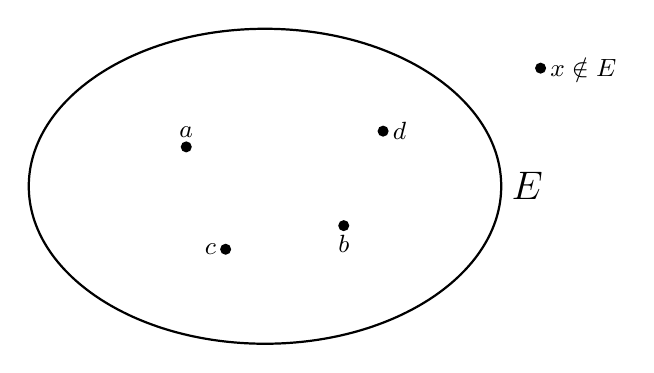
\begin{tikzpicture}
        % Dessin de l'ensemble E
        \draw[thick] (0,0) ellipse (3 and 2) node[right=3cm] {\Large $E$};
        
        % Points représentant des éléments quelconques
        \fill (-1,0.5) circle (2pt) node[above] {\small $a$};
        \fill (1,-0.5) circle (2pt) node[below] {\small $b$};
        \fill (-0.5,-0.8) circle (2pt) node[left] {\small $c$};
        \fill (1.5,0.7) circle (2pt) node[right] {\small $d$};
        
        % Un élément extérieur à E
        \fill (3.5,1.5) circle (2pt) node[right] {\small $x \notin E$};

    \end{tikzpicture}
\end{center}
\subsection{Ensembles élémentaires :}
Il y a plusieurs ensembles de bases importantes à connaître.
\begin{mdframed}
    \[
\begin{aligned}
    \mathbb{N} &= \{0, 1, 2, 3, \dots\} \quad &&\text{(Ensemble des entiers naturels)} \\
    \mathbb{Z} &= \{\dots, -2, -1, 0, 1, 2, \dots\} \quad &&\text{(Ensemble des entiers relatifs)} \\
    \mathbb{Q} &= \left\{ \frac{a}{b} \mid a \in \mathbb{Z}, b \in \mathbb{Z}^* \right\} \quad &&\text{(Ensemble des nombres rationnels)} \\
    \mathbb{R} &= \{0;1;-4;\frac{68}{97}; 78,23456...;\pi;\sqrt{2};...\}\quad &&\text{(Ensemble des nombres réels)} \\
    \mathbb{C} &= \{ a + bi \mid a, b \in \mathbb{R}, i^2 = -1 \} \quad &&\text{(Ensemble des nombres complexes)} \\
    \mathbb{K}(i)&=\{k_1+ik_2\: |\: k_1,k_2\in \mathbb{K},i^2=-1\}\\
    \mathbb{P} &= \{2, 3, 5, 7, 11, 13, \dots\} \quad &&\text{(Ensemble des nombres premiers)} \\
    \varnothing &= \{\} \quad &&\text{(Ensemble vide)}
\end{aligned}
\]
\end{mdframed}
Il y a aussi des ensembles de matrices de bases
\begin{mdframed}
\[
\begin{aligned}
    M_{n}^m(\mathbb{K}) &= \{ A \mid A \text{ est une matrice de dimensions } m \times n \text{ à coefficients dans } \mathbb{K} \} \\
    M_n(\mathbb{K}) &= \{ A \mid A \text{ est une matrice carrée } n \times n \text{ sur } \mathbb{K} \} \\
    GL_n(\mathbb{K}) &= \{ A \mid A \in M_n(\mathbb{K}), \det(A) \neq 0 \}
\end{aligned}
\]
\end{mdframed}

\subsection{Opérations ensemblistes}


    \begin{definition}[Égalité]
        Soient $A$, $B$ deux ensembles. On dit que $A$ et $B$ sont égaux ce qu'on note $A=B$ si
        \[
        \forall x \quad (x\in A)\Leftrightarrow(x\in B)
        \]
    \end{definition}

Autrement dit $A=B$ si et seulement si $A$ et $B$ contiennent exactement les mêmes objets.\\
\textbf{Exemple :}
\[
\{0,2,4,6\}=\{6,2,0,4\}=\{2k\;|\;k\in \{0,1,2,3\}\}
\]

    \begin{definition}[Inclusion]
    Soient $A,B$ des ensembles. On dit que $A$ est inclus a $B$. Ce que l'on note $A\subseteq B$ si 
    \[
    \forall x \quad (x\in A)\Rightarrow(x\in B)
    \]
    \end{definition}

Si $A$ est inclus dans $B$, cela signifie que tous les éléments de $A$ sont contenus dans $B$.
\begin{exemple}
    \[
\{1,3\}\subseteq \{0,1,2,3,4\}
\]
On a aussi l'inclusion stricte, $\subset$, qui garantit que $A$ est différent de $B$.
\end{exemple}


\begin{center}
    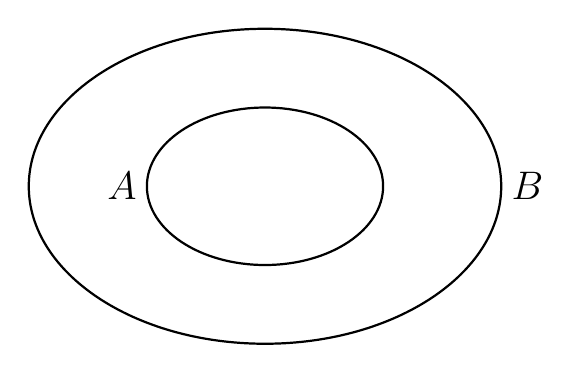
\begin{tikzpicture}
        % Ensemble B (plus grand)
        \draw[thick] (0,0) ellipse (3 and 2) node[right=3cm] {\Large $B$};
        
        % Ensemble A (inclus dans B)
        \draw[thick] (0,0) ellipse (1.5 and 1) node[left=1.5cm] {\Large $A$};
    \end{tikzpicture}
\end{center}

\begin{remarque}
    Nous avons les propriétés suivantes
    \begin{align*}
        &\forall A, \quad &&A \subseteq A\\
        &\forall A,B,C, \quad &&((A\subseteq B) \wedge(B\subseteq C)) \Rightarrow (A\subseteq C)\\
        &\forall A,B, \quad &&((A\subseteq B)\wedge(B\subseteq A)) \Rightarrow (A=B)
    \end{align*}
\end{remarque}



\begin{definition}[Intersection]
    Soient $A,B$ des ensembles. On définit l'intersection de $A$ et $B$ comme l'ensemble
    \[
    A\cap B=\{x\: |\: x\in A \wedge x\in B\}
    \]
\end{definition}
L'intersection de $A$ et $B$ est l'ensemble des éléments qui appartiennent à $A$ et $B$\\
\textbf{Exemple :}\\
\[
\{0,1,2,10\}\cap\{\pi,0,4,2\}=\{0,2\}
\]
\begin{center}
    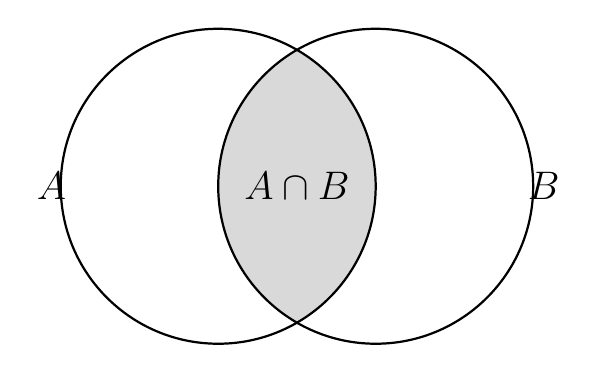
\begin{tikzpicture}
        % Deux cercles se chevauchant
        \begin{scope}
            \clip (0,0) circle (2);
            \fill[gray!30] (2,0) circle (2);
        \end{scope}
        
        % Cercle A
        \draw[thick] (0,0) circle (2) node[left=1.8cm] {\Large $A$};
        
        % Cercle B
        \draw[thick] (2,0) circle (2) node[right=1.8cm] {\Large $B$};
        
        % Marquer l'intersection
        \node at (1,0) {\Large $A \cap B$};
    \end{tikzpicture}
\end{center}
\begin{remarque}
    Soient $A,B$ des ensembles. On a
    \[
    A\cap B=A \: \Leftrightarrow \: B\subseteq A
    \]
\end{remarque}

    \begin{definition}[Union]
        Soient $A,B$ des ensembles. On définit l'union de $A$ et $B$ comme l'ensemble
        \[
        A\cup B=\{x\:|\: x\in A \vee x\in B\}
        \]
    \end{definition}
\textbf{Exemple :}\\
\[
\{0,1,2,10\}\cup\{\pi,0,4,2\}=\{0,1,2,\pi,4,10\}
\]

\begin{center}
    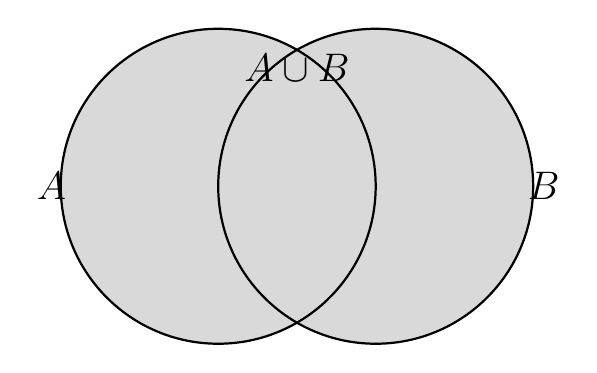
\begin{tikzpicture}
        % Remplissage de l'union
        \begin{scope}
            \fill[gray!30] (0,0) circle (2);
            \fill[gray!30] (2,0) circle (2);
        \end{scope}
        
        % Cercle A
        \draw[thick] (0,0) circle (2) node[left=1.8cm] {\Large $A$};
        
        % Cercle B
        \draw[thick] (2,0) circle (2) node[right=1.8cm] {\Large $B$};
        
        % Marquer l'union
        \node at (1,1.5) {\Large $A \cup B$};
    \end{tikzpicture}
\end{center}

\begin{remarque} Nous avons la distributivité avec ces opérations.
    \[
A \cap (B \cup C) = (A \cap B) \cup (A \cap C)
\]
\[
A \cup (B \cap C) = (A \cup B) \cap (A \cup C)
\]
\end{remarque}


    \begin{definition}[Soustraction]
        Soient $A,B$ deux ensembles. On définit l'ensemble $A$ privé de $B$ comme
        \[
        A \setminus B=\{x\:| x\in A \wedge x\notin B\}
        \]
    \end{definition}



\begin{center}
    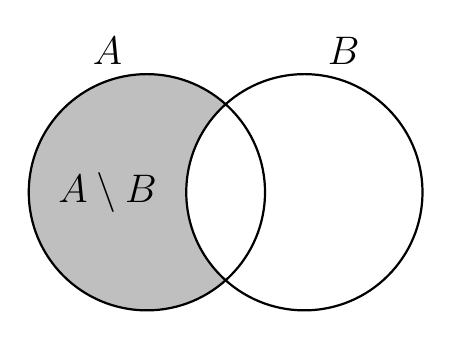
\begin{tikzpicture}
        % Remplissage de A privé de B en gris
        \begin{scope}
            \clip (-1,0) circle (1.5); % Garde seulement A
            \fill[gray!50] (-3,-2) rectangle (3,2); % Remplit toute la zone
        \end{scope}
        \begin{scope}
            \clip (1,0) circle (1.5); % Enlève B du remplissage
            \fill[white] (-3,-2) rectangle (3,2);
        \end{scope}

        % Dessiner les cercles A et B
        \draw[thick] (-1,0) circle (1.5);
        \draw[thick] (1,0) circle (1.5);

        % Placer correctement les labels
        \node at (-1.5,0) {\Large $A \setminus B$}; % Bien placé dans la zone blanche de A
        \node at (-1.5,1.8) {\Large $A$}; % Remonté au-dessus du cercle A
        \node at (1.5,1.8) {\Large $B$}; % Remonté au-dessus du cercle B
    \end{tikzpicture}
\end{center}




    \begin{definition}[Complémentaire]
        Soit $A$ un ensemble. On définit le complémentaire de $A$ comme l'ensemble
        \[
        A^{\complement}=\mathcal{C}(A)=\{x\: |\: x\notin A\}
        \]
    \end{definition}

\begin{exemple}
    Le complémentaire de $\mathbb{N}$ dans $\mathbb{Z}$ est l'ensemble $\{-1,-2,-3,...\}$.
\end{exemple}

 
\begin{center}
    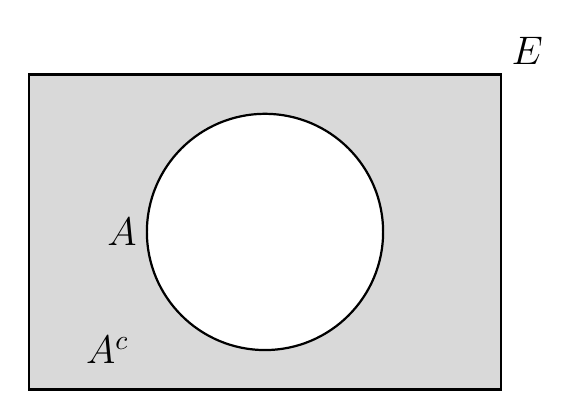
\begin{tikzpicture}
        % Ensemble universel E (rectangle)
        \fill[gray!30] (-3,-2) rectangle (3,2); % Remplissage gris pour A^c
        \draw[thick] (-3,-2) rectangle (3,2) node[above right] {\Large $E$};

        % Ensemble A (blanc)
        \fill[white] (0,0) circle (1.5); % A reste blanc
        \draw[thick] (0,0) circle (1.5) node[left=1.5cm] {\Large $A$};

        % Marquer le complémentaire de A
        \node at (-2,-1.5) {\Large $A^c$};

    \end{tikzpicture}
\end{center}

    \begin{definition}
        Soient $A,B$ des ensembles. On dit que $A$ est une partie de l'ensemble $B$ si $A\subseteq B$. L'ensemble de toutes les parties de $B$ est noté $\mathcal{P}(B)$
        \[
        \mathcal{P}(B)=\{A \: |\: A\subseteq B\}
        \]
    \end{definition}
\begin{exemple}
    \[
\partie(\{1,2,3\})= \{ \varnothing, \{1\}, \{2\}, \{3\}, \{1,2\}, \{1,3\}, \{2,3\}, \{1,2,3\} \}
\]
\end{exemple}

\begin{remarque}
    Soient $A,B$ des ensembles
    \[
    A\subseteq B \Leftrightarrow A\in \mathcal{P}(B)
    \]
\end{remarque}
\begin{exercice}
Démontrer les lois de Morgan
\[
(A \cup B)^{\complement} = A^{\complement}\cap B^{\complement}
\]
\[
(A \cap B)^{\complement} = A^{\complement} \cup B^{\complement}
\]
\end{exercice}


\subsection{Relations et fonctions}



\begin{definition} 
Une \textbf{relation binaire} entre les éléments de \( A \) et les éléments de \( B \) est un sous-ensemble de \( A \times B \) pouvant être représenté par un ensemble de flèches reliant les éléments de \( A \) aux éléments de \( B \).  
\end{definition}


\begin{center} % Centrer tout le diagramme
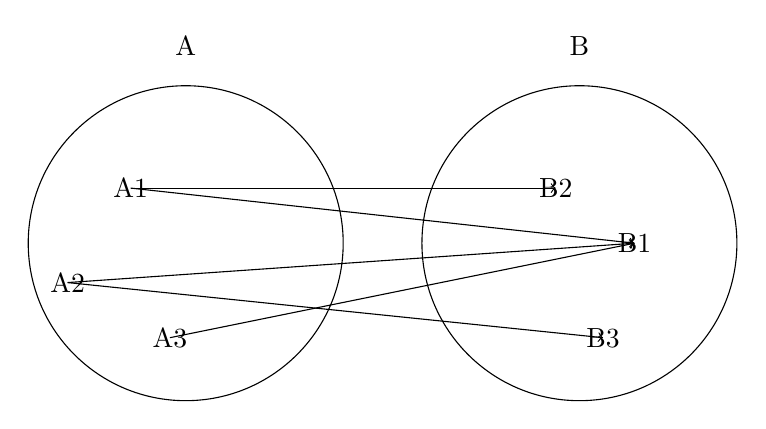
\begin{tikzpicture}

% Ensemble A (cercle à gauche)
\draw (0,0) circle (2cm);
\node at (0, 2.5) {A};

% Ensemble B (cercle à droite)
\draw (5,0) circle (2cm);
\node at (5, 2.5) {B};

% Élément A1, A2, A3 dans A
\node at (-0.7, 0.7) {A1};
\node at (-1.5, -0.5) {A2};
\node at (-0.2, -1.2) {A3};

% Élément B1, B2, B3 dans B
\node at (5.7, 0) {B1};
\node at (4.7, 0.7) {B2};
\node at (5.3, -1.2) {B3};

% Flèches représentant la relation R (de A vers B)
\draw[->] (-0.7, 0.7) -- (5.7, 0);  % A1 -> B1
\draw[->] (-1.5, -0.5) -- (5.7, 0); % A2 -> B1
\draw[->] (-0.2, -1.2) -- (5.7, 0); % A3 -> B1

% Flèches supplémentaires pour illustrer d'autres relations
\draw[->] (-0.7, 0.7) -- (4.7, 0.7);  % A1 -> B2
\draw[->] (-1.5, -0.5) -- (5.3, -1.2); % A2 -> B3

\end{tikzpicture}
\end{center}
\textbf{Exemples :}\\
\[
=_{\mathbb{R}}:\{(r_1,r_2)\in \mathbb{R}^2\:|\:r_1=r_2\}
\]
\[
\leq_{\mathbb{R}}:\{ (r_1,r_2)\in \mathbb{R}^2 \: |\: r_1\leq r_2 \}
\]
Suite à cette définition, il est naturel de définir les ensembles suivants pour étudier les propriétés des relations.
\begin{definition} 
Soit \( R \subset A \times B \) une relation.  

\begin{itemize}
    \item Le \textbf{domaine} de \( R \), noté \( \text{dom} R \), est le sous-ensemble de \( A \) défini par :  
    \[
    \text{dom} R = \{ a \in A \mid \exists b \in B, (a, b) \in R \}
    \]
    (C'est-à-dire, l'ensemble des éléments de \( A \) ayant une flèche sortante).
    
    \item L'\textbf{image} de \( R \), notée \( \text{Im} R \), est le sous-ensemble de \( B \) défini par :  
    \[
    \text{Im} R = \{ b \in B \mid \exists a \in A, (a, b) \in R \}
    \]
    (C'est-à-dire, l'ensemble des éléments de \( B \) ayant une flèche entrante).
\end{itemize}
\end{definition}

\begin{definition}   

    \item Une \textbf{fonction} de \( A \to B \) est une relation \( F \subset A \times B \) telle que \( \forall a \in A \), il existe au plus un élément de \( B \) tel que \( (a, b) \in F \).  
    \item \(F \) est une \textbf{fonction} de \( A \to B \) si :
    \[
    \forall a \in A, \exists ! b \in B \text{ tel que } (a, b) \in F.
    \]
    De plus, on dira que $F$ est une application si $A=dom(f)$.
\end{definition}
Soit $f:\R \to \R :x\mapsto x^2$. On a $\dom(f)= \mathbb{R}$, $f$ est donc une application. De plus, $\im(f)=\mathbb{ R}^{\geq 0}$.
\begin{exemple}
    
\end{exemple}


\begin{definition}
Soit \( R \) une relation entre deux ensembles \( A \) et \( B \). La relation inverse \( R^{-1} \) est définie comme suit :

\[
R^{-1} \subseteq B \times A
\]

Plus précisément, si \( (a, b) \in R \), alors \( (b, a) \in R^{-1} \). En d'autres termes, la relation inverse consiste à inverser chaque paire de la relation \( R \).

Formellement, si \( R \subseteq A \times B \), alors la relation inverse \( R^{-1} \subseteq B \times A \) est donnée par :

\[
R^{-1} = \{ (b, a) \mid (a, b) \in R \}
\]
\end{definition}
Ainsi $R^{-1}$ est l'inverse de $R$, voici un exemple l'illustrant:\\

\begin{exemple}
    On note la fonction identité $id_\mathbb{R}:\mathbb{R}\to \mathbb{R},\: x\mapsto x$. \\
Soit $f:\mathbb{R} \to \mathbb{R}, \: x\mapsto x+1 $
et soit $g: \mathbb{R \to \mathbb{R}}, \: x\mapsto x -1$.\\
Remarquons que nous avons
\[
f \circ g=g\circ f=id_{\mathbb{R}}
\]
c'est à dire que pour tout $x\in \mathbb{R}$, on a
\[
f(g(x))=f(x-1)=x-1+1=x=x+1-1=g(x-1)=g(f(x))
\]
\end{exemple}

\begin{exemple}
    Soit \( A = \{1, 2, 3\} \) et \( B = \{a, b, c\} \), et supposons que la relation \( R \subseteq A \times B \) soit définie par :

\[
R = \{(1, a), (2, b), (3, c)\}
\]

L'inverse de cette relation \( R^{-1} \) sera :

\[
R^{-1} = \{(a, 1), (b, 2), (c, 3)\}
\]
\end{exemple}


    

\begin{definition}
    Une fonction \( F : A \to B \) est dite \textbf{injective} (ou \textbf{injection}) si elle envoie des éléments distincts de \( A \) sur des éléments distincts de \( B \), c'est-à-dire :
\[
\forall a_1, a_2 \in A, \quad F(a_1) = F(a_2) \Rightarrow a_1 = a_2.
\]
Autrement dit, chaque élément de \( B \) est l'image d'au plus un élément de \( A \).
Et elle est dites \textbf{surjective} (ou \textbf{surjection}) si tout élément de \( B \) possède au moins un antécédent dans \( A \), c'est-à-dire :
\[
\forall b \in B, \quad \exists a \in A \text{ tel que } F(a) = b.
\]
Autrement dit, l'image de \( f \) est \( B \), soit \( \text{Im}(F) = B \)\\
Une fonction injective et surjective est dites \textbf{bijective}.

\end{definition}

La notion d'injectivité est nous donne la propriété que $F$ est une correspondance "one to one". En terme de flèches, chaque éléments de $\dom(f)$ est relié à un seul élément de $Im(f)$.

\begin{definition}
    On note l'ensemble des fonctions bijectives de $X$ dans $X$, $\mathfrak{S}(X)$
\end{definition}

\begin{proposition}
    Soit $F$ une fonction bijective alors $F^{-1}$ est bijective.
\end{proposition}

\begin{proof}
    Soit \( F : A \to B \) une fonction bijective, c'est-à-dire que \( F \) est injective et surjective. Nous devons prouver que \( F^{-1} : B \to A \) est également bijective, c'est-à-dire qu'elle est injective et surjective.

\medskip
\textbf{1. Injectivité de \( F^{-1} \) :}

Soit \( y_1, y_2 \in B \) tels que \( F^{-1}(y_1) = F^{-1}(y_2) \). Nous devons montrer que \( y_1 = y_2 \).

\begin{itemize}
    \item Par définition de \( F^{-1} \), \( F^{-1}(y_1) = x_1 \) et \( F^{-1}(y_2) = x_2 \), où \( F(x_1) = y_1 \) et \( F(x_2) = y_2 \).
    \item Supposons que \( F^{-1}(y_1) = F^{-1}(y_2) \), cela signifie que \( x_1 = x_2 \).
    \item Comme \( F \) est injective, \( F(x_1) = F(x_2) \) implique que \( x_1 = x_2 \). Ainsi, \( y_1 = y_2 \).
\end{itemize}

Donc, \( F^{-1} \) est injective.

\medskip
\textbf{2. Surjectivité de \( F^{-1} \) :}

Soit \( x \in A \). Nous devons montrer qu'il existe un \( y \in B \) tel que \( F^{-1}(y) = x \).

\begin{itemize}
    \item Par définition de \( F^{-1} \), \( F^{-1}(y) = x \) signifie que \( F(x) = y \).
    \item Comme \( F \) est surjective, pour chaque \( x \in A \), il existe un \( y \in B \) tel que \( F(x) = y \). Donc, \( F^{-1}(y) = x \).
\end{itemize}

Donc, \( F^{-1} \) est surjective.
\end{proof}


\subsection{Courbes de niveau}
    

\begin{definition} 
Soit \( F \) une fonction de \( A \to B \) et soit $b\in B$ 

On appelle \textbf{courbes de niveau} de \( F \) l’ensemble :  
  \[
  C_b (F)= \{ a \in A \mid F(a) = b \}
  \]
\end{definition}
\begin{remarque}On a
    
\begin{enumerate}
    \item \( F \) est \textbf{surjective} si \( \forall b \in B \), \( C_b (F) \neq \emptyset \).
    \item \( F \) est \textbf{injective} si \( \forall b \in \text{Im} F \), \( C_b (F) \) est un singleton.
\end{enumerate}
\end{remarque}

\begin{proposition}
    Soit $b,b'\in B$ et soient \( C_b (F) \) et \( C_{b'} (F) \) deux courbes de niveau de \( F \), alors soit elles sont \textbf{confondues}, soit elles sont \textbf{disjointes}.
\end{proposition} 

\begin{proof}
Soit \( x \in C_b(F) \cap C_{b'}(F) \), c'est-à-dire un élément appartenant à l'intersection des deux courbes de niveau. Par définition de ces ensembles, on a :
\[
F(x) = b \quad \text{et} \quad F(x) = b'.
\]
En conséquence, on obtient :
\[
b = b'.
\]

Cela signifie que si l'intersection \( C_b(F) \cap C_{b'}(F) \) est non vide, alors nécessairement \( b = b' \), ce qui implique que :
\[
C_b(F) = C_{b'}(F).
\]

Dans le cas contraire, si \( b \neq b' \), alors il n'existe aucun \( x \in A \) tel que \( F(x) = b \) et \( F(x) = b' \) simultanément, ce qui entraîne :
\[
C_b(F) \cap C_{b'}(F) = \emptyset.
\]
\end{proof}

\begin{remarque}
    On a donc que une fonction est injective si et seulement si toutes ses courbes de niveau sont des singletons.
\end{remarque}













\section{Arithmétique}
Dans ce chapitre, nous allons voir des résultats fondamentaux en arithmétique qui nous seront plus qu'utile dans grand nombre de preuve. Voyez ce chapitre comme une introduction à l’arithmétique.
\subsection{Division Euclidienne}

\begin{theoreme}[Division euclidienne]
    Soient $m$ et $n$ des entiers positifs, et m non nul. Il existe alors des entiers $q$ et $r$ positif, avec $0\leq r<m$ tels que
    \[
    n=qm +r
    \]
    Les entiers $q$ et $r$ sont déterminés de manière unique par ces conditions.
\end{theoreme}

\begin{proof}
    Démontrons l'existence de ces entiers par récurrence sur n.
    \\ Si $n=0$, nous posons $q=r=0. $ Supposons $n>0$. Si $n<m$, nous posons encore $q=0$ et $r=n$. Si $n\geq m$, alors $0\leq n-m<n$. Par hypothèse de récurrence, on peut trouver des entiers $q_1$ et $r$ positifs ou nuls tels que
    \[
    n-m=q_1m+r
    \]
    alors \[
    n=m+q_1m+r=(1+q_1)m +r
    \]
    On a ainsi démontré l'existence des entiers $q$ et $r$ recherchés. Quant à l'unicité, supposons que
    \begin{align*}
        &n=q_1m+r_1, \quad 0\leq r_1<m\\
        &n=q_2m+r_2, \quad 0\leq r_2<m
    \end{align*}
    Si $r_1\neq r_2$, par exemple si $r_2>r_1$, nous obtenons par soustraction
    \[
    (q_1-q_2)m= r_2-r_1.
    \]
    Mais $r_2-r_1<m$ et $r_2-r_1>0$. Cela est impossible puisque $q_1-q_2$ est un entier, et qu'ainsi $(q_1-q_2)m>0$ implique $(q_1-q_2)m>m$. Nous en déduisons que $r_1=r_2$. Mais alors $q_1m=q_2m$, donc $q_1=q_2$. ce qui prouve l'unicité, et achève la démonstration.
\end{proof}
\subsection{Plus grand commun diviseur}

\begin{definition}
    Soient $n$ et $d$ des entiers non nuls. Nous disons que $d$ divise $n$ si
    \[
    \exists q\in \mathbb{Z}, \quad n=dq
    \]
    Nous écrivons alors $d\mid n$.
\end{definition}
\begin{definition}
    Un \textit{nombre premier} est un naturel \( p \) supérieur à 1 qui n'admet que deux diviseurs distincts : 1 et lui-même. Autrement dit, \( p \) est premier si et seulement si :  

\[
\forall d \in \mathbb{N}, \quad d \mid p \Rightarrow (d = 1 \text{ ou } d = p).
\]
\end{definition}

\begin{definition}
   Si $a,b\in \mathbb{Z}$ sont non nuls, alors  le plus grand commun diviseur (PGCD) de $a$ et $b$ est le nombre $d$ strictement positif satisfaisant :
   \begin{enumerate}
       \item $d\mid a$ et $d\mid b$;
       \item si $c\mid a$ et $c\mid b$, alors $c\leq d$.
   \end{enumerate}
   Ce nombre est noté $\text{pgcd}(a,b)$
\end{definition}

\begin{definition}
    Deux entiers \( a \) et \( b \) sont dits \textbf{premiers entre eux} si leur seul diviseur commun est 1, c'est-à-dire si leur plus grand commun diviseur (PGCD) est égal à 1 :  

\[
\text{pgcd}(a, b) = 1.
\]
\end{definition}

\begin{definition}
    Pour tous $a,b\in \mathbb{Z}_0$, on définit l'ensemble
    \[
    E_{a,b}=\{c\in \mathbb{Z}\mid c>0, c\mid a\\ \mathrm{\ et\ } c\mid b\}
    \]
\end{definition}

\begin{proposition}
    Si $a,b\in \mathbb{Z}$ sont non nuls, alors le plus grand diviseur de $a$ et $b$ existe et est unique.
\end{proposition}

\begin{proof}
    Pour tous $a,b\in \mathbb{Z}_0$, $E_{a,b}$ est non vide car il contient $1$. Donc Il a un un maximum et il est unique. 
\end{proof}

\begin{proposition}
    Pour tous $a,b\in \mathbb{Z}_0$, on a
    \[
    \text{pgcd}(a,b)=\text{pgcd}(-a,b)=\text{pgcd}(a,-b)=\text{pgcd}(-a,-b)
    \]
\end{proposition}

\begin{proof}
    On démontre par double inclusion que les ensembles $E_{a,b},E_{-a,b},E_{a,-b},$\\$E_{-a,-b}$ sont égaux. Cela vient du fait que si un nombre $c$ divise un nombre $a$, il divise aussi $-a$.
\end{proof}

\begin{proposition}
Pour tous \( a, b \in \mathbb{Z}_0 \) et tout \( m \in \mathbb{Z} \), on a 
\[
\text{pgcd}(a,b) = \text{pgcd}(a, b + ma).
\]
\end{proposition}

\begin{proof}
On prouve ici encore que les ensembles \( E_{a,b} \) et \( E_{a,b+ma} \) coïncident, par double inclusion.  
Soit \( c \in E_{a,b} \). Par définition, il existe \( k, k' \in \mathbb{Z} \) tels que \( a = kc \) et \( b = k'c \).  
Alors \( b + ma = k'c + mkc = (k' + mk)c \) et \( c \) divise ainsi \( a \) et \( b + ma \).  
On a donc démontré \( E_{a,b} \subset E_{a,b+ma} \).  

Pour l’autre inclusion, si \( c \) appartient à \( E_{a,b+ma} \), il existe \( k, k' \in \mathbb{Z} \) tels que \( a = kc \) et \( b + ma = k'c \).  
On a alors \( b = (k' - mk)c \) et \( c \) appartient à \( E_{a,b} \).  
\end{proof}

\begin{proposition}[Algorithme d'Euclide]
Soient deux nombres entiers \( a, b \) tels que \( b > a > 0 \).  
On pose \( a = r_0 \) et on écrit la suite de divisions :
\[
\begin{aligned}
    b &= q_1 a + r_1 \\
    a &= q_2 r_1 + r_2 \\
    r_1 &= q_3 r_2 + r_3 \\
    &\vdots \\
    r_{j-1} &= q_{j+1} r_j + r_{j+1} \\
    &\vdots \\
    r_{j-1} &= q_{j+1} r_j + 0.
\end{aligned}
\]
Alors le dernier reste non nul \( r_j \) est le pgcd de \( a \) et \( b \).
\end{proposition}

\begin{proof}
Tout d'abord, la suite des restes est formée de nombres entiers positifs et est strictement décroissante. Elle atteint donc 0 et il y a toujours un \( J \geq 0 \) tel que \( r_{J+1} = 0 \).  
La procédure de calcul est donc bien définie. Montrons qu'elle conduit au bon résultat.  

Par la proposition précédente, puisque \( r_1 = b - q_1 a \), on a \( \text{pgcd}(a, b) = \text{pgcd}(a, r_1) \).  
On montre de la même façon que \( \text{pgcd}(r_{j-1}, r_j) = \text{pgcd}(r_{j+1}, r_j) \) pour \( j \in \{1, \dots, J-1\} \),  
puisque \( r_{j+1} = r_{j-1} - q_j r_j \).  

Cette suite d’égalités montre que le pgcd de \( a \) et \( b \) est le pgcd de \( r_{J-1} \) et \( r_J \),  
qui est \( r_J \), puisque \( r_J \) divise \( r_{J-1} \).
\end{proof}


\begin{theoreme}[Bézout]
Si \( a, b \in \mathbb{Z} \) sont non nuls et si \( d = \text{pgcd}(a, b) \), alors il existe \( x_0, y_0 \in \mathbb{Z} \) tels que  
\[
d = ax_0 + by_0.
\]
\end{theoreme}

\begin{proof}
On considère l’ensemble 
\[
S = \{ax + by \mid x, y \in \mathbb{Z} \text{ et } ax + by > 0\}.
\]
Cet ensemble est formé de nombres entiers strictement positifs, il est donc inclus dans \( \mathbb{N} \).  
Cet ensemble est non vide, car il contient \( a \) si \( a > 0 \), ou \( -a \) si \( a < 0 \).  

Puisque \( \mathbb{N} \) est bien ordonné, \( S \) admet un élément minimal, que nous notons \( c \). Montrons que \( c \) est le pgcd de \( a \) et \( b \).  
Par définition, il existe \( x_0, y_0 \in \mathbb{Z} \) tels que \( c = ax_0 + by_0 \).  

On montre que \( c \) divise \( a \) par l’absurde. Supposons que \( c \) ne divise pas \( a \),  
la division de \( a \) par \( c \) s’écrit
\[
a = q c + r, \quad 0 < r < c.
\]
Alors on a \( r < c \) et \( r \) appartient à \( S \), ce qui est absurde.  
On a en effet \( r > 0 \) et \( r = a - qc = a - q(ax_0 + by_0) = (1-qx_0)a + b(-qy_0) \).  

On montre de la même manière que \( c \) divise \( b \).  
On montre ensuite que \( c \) est le plus grand diviseur commun de \( a \) et \( b \).  
En effet, si \( d \) divise \( a \) et \( b \), soit \( c \leq 0 \), soit \( c > 0 \).  

Dans le second cas, \( d \) divise \( ax_0 + by_0 \), donc \( c \leq d \).
\end{proof}

\begin{corollaire}
    $\forall a,b \in \mathbb{Z}_0$ $a$ et $b$ sont premiers entre eux si et seulement si il existe $x_0,y_0\in \mathbb{Z}_0$ tels que 
    \[
    1=ax_0+by_0
    \]
\end{corollaire}

\begin{proof}
    Par le théorème de Bézout, $\operatorname{pgcd}(a,b)=1$ donc par définition $a$ et $b$ sont premiers entre eux
\end{proof}

\begin{lemme}[Gauss]
Soient \( a, b, c \) trois entiers. Si \( a \) divise \( bc \) et est premier avec \( b \), alors \( a \) divise \( c \).
\end{lemme}

\begin{proof}
    Puisque \( a \) est premier avec \( b \), il existe, d'après le théorème de Bézout, deux entiers \( x \) et \( y \) tels que :
\[
ax + by = 1.
\]
En multipliant cette égalité par \( c \), on obtient :
\[
acx + bcy = c.
\]
Comme \( a \) divise \( bc \), il existe un entier \( k \) tel que \( bc = ak \). En remplaçant dans l’égalité précédente, on obtient :
\[
acx + a(ky) = c.
\]
On peut factoriser \( a \) :
\[
a(cx + ky) = c.
\]
Ainsi, \( a \) divise \( c \), ce qui conclut la démonstration.
\end{proof}
\subsection{Décomposition en facteur premier}


\begin{lemme}[Euclide]
Soit $p$ un nombre premier et soit $m$ et $n$ des entiers non nuls tel que $p\mid mn$ alors $p\mid m$ ou $p\mid n$.
\end{lemme}

\begin{proof}
Supposons que \( p \) ne divise pas \( m \). Puisque \( p \) est premier et que \( p \nmid m \), cela signifie que \( p \) et \( m \) sont premiers entre eux, c'est-à-dire que :
\[
\operatorname{pgcd}(p, m) = 1.
\]
D'après le théorème de Bézout, il existe alors deux entiers \( x \) et \( y \) tels que :
\[
px + my = 1.
\]
En multipliant cette égalité par \( n \), on obtient :
\[
p(xn) + m(yn) = n.
\]
Or, par hypothèse, \( p \mid mn \), donc \( p \mid m(yn) \). Comme \( p \) divise aussi \( p(xn) \), il en résulte que \( p \) divise la somme :
\[
p(xn) + m(yn) = n.
\]
Ainsi, \( p \mid n \), ce qui conclut la démonstration.
\end{proof}

    

\begin{theoreme}
    Tout nombre naturel supérieur ou égale à $2$ se décompose en un produit de facteurs premiers. La décomposition est unique à l'ordre des facteur près.
\end{theoreme}

\begin{proof}
\textbf{Existence :} Nous procédons par récurrence sur \( n \).

- Pour \( n = 2 \), qui est un nombre premier, la propriété est triviale.
- Supposons que tout entier \( k \) tel que \( 2 \leq k \leq n \) puisse être écrit comme un produit de nombres premiers.
- Considérons \( n+1 \) :
  - Si \( n+1 \) est premier, il est déjà sous la forme voulue.
  - Sinon, il existe deux entiers \( a \) et \( b \) tels que \( n+1 = a \cdot b \) avec \( 2 \leq a, b < n+1 \).
  - Par hypothèse de récurrence, \( a \) et \( b \) se décomposent en facteurs premiers, et donc \( n+1 \) aussi.

Par récurrence, tout entier \( n \geq 2 \) admet une décomposition en facteurs premiers.

\textbf{Unicité :} Supposons qu'il existe deux décompositions distinctes d'un même entier \( n \) :
\[
n = p_1 p_2 \dots p_k = q_1 q_2 \dots q_m
\]
où \( p_i \) et \( q_j \) sont des nombres premiers. Comme \( p_1 \) divise \( q_1 q_2 \dots q_m \) et qu'il est premier, il doit diviser l'un des \( q_j \). Or, les \( q_j \) sont premiers, donc \( p_1 = q_j \). En annulant ce facteur de chaque côté, on applique la même argumentation aux autres facteurs, ce qui montre que les ensembles \( \{p_1, p_2, \dots, p_k\} \) et \( \{q_1, q_2, \dots, q_m\} \) sont identiques, à l'ordre près.

Ainsi, la décomposition en facteurs premiers est unique à l'ordre près, ce qui conclut la démonstration.
\end{proof}
\subsection{Plus petit commun multiple}

\begin{definition}
    Soient \( a, b \) deux entiers naturels non nuls. Le \textbf{Plus Petit Commun Multiple (PPCM)} de \( a \) et \( b \), noté \( \operatorname{ppcm}(a, b) \), est défini comme l'unique entier \( m \) vérifiant les conditions suivantes :
    \begin{enumerate}
        \item \( m \) est un multiple commun de \( a \) et \( b \) :
        \[
        a \mid m \quad \text{et} \quad b \mid m
        \]
        c'est-à-dire que \( m \) est divisible par \( a \) et par \( b \).
    
        \item \( m \) est le plus petit parmi ces multiples :
        \[
        \forall n \in \mathbb{N}, \quad (a \mid n \text{ et } b \mid n) \Rightarrow m \leq n.
        \]
        Autrement dit, si \( n \) est un autre multiple commun de \( a \) et \( b \), alors \( m \) est inférieur ou égal à \( n \).
    \end{enumerate}
\end{definition}

\begin{exemple}
    Calculons le \textbf{PPCM} de \( 36 \) et \( 48 \).
    
    Étape 1 : Décomposition en facteurs premiers
    \[
    36 = 2^2 \times 3^2, \quad 48 = 2^4 \times 3^1
    \]
    
    Étape 2 : Détermination du PPCM
    
    Le PPCM est obtenu en prenant les \textbf{plus grandes puissances} de chaque facteur premier :
    
    \[
    \operatorname{PPCM}(36, 48) = 2^4 \times 3^2
    \]
    
    Donc
    
    \[
    \operatorname{PPCM}(36, 48) = 16 \times 9 = 144
    \]
\end{exemple}

\begin{proposition}
    Pour tous entiers naturels non nuls \( a, b \), on a la relation :
    \[
     \operatorname{pgcd}(a, b) \cdot\operatorname{ppcm}(a, b) = a\cdot b
    \]
\end{proposition}

\begin{proof}
    Soient \( a, b \) deux entiers naturels non nuls. Décomposons-les en facteurs premiers :
    \[
    a = p_1^{\alpha_1} p_2^{\alpha_2} \dots p_k^{\alpha_k}, \quad 
    b = p_1^{\beta_1} p_2^{\beta_2} \dots p_k^{\beta_k}.
    \]
    
    Le **PGCD** est donné par :
    \[
    \operatorname{pgcd}(a, b) = p_1^{\min(\alpha_1, \beta_1)} p_2^{\min(\alpha_2, \beta_2)} \dots p_k^{\min(\alpha_k, \beta_k)}.
    \]
    
    Le **PPCM** est donné par :
    \[
    \operatorname{ppcm}(a, b) = p_1^{\max(\alpha_1, \beta_1)} p_2^{\max(\alpha_2, \beta_2)} \dots p_k^{\max(\alpha_k, \beta_k)}.
    \]
    
    On vérifie que :
    \[
    \operatorname{pgcd}(a, b) \cdot \operatorname{ppcm}(a, b) = 
    \left( p_1^{\min(\alpha_1, \beta_1)} \dots p_k^{\min(\alpha_k, \beta_k)} \right)
    \cdot
    \left( p_1^{\max(\alpha_1, \beta_1)} \dots p_k^{\max(\alpha_k, \beta_k)} \right).
    \]
    
    Or, pour tout \( i \), on a :
    \[
    \min(\alpha_i, \beta_i) + \max(\alpha_i, \beta_i) = \alpha_i + \beta_i.
    \]
    
    Ainsi, on retrouve bien la décomposition de \( a \times b \), ce qui prouve la relation :
    \[
    a \cdot b = \operatorname{pgcd}(a, b) \cdot \operatorname{ppcm}(a, b).
    \]
\end{proof}
\subsection{Théorème de Fermat-Wiles }
\begin{theoreme}[Fermat-Wiles]
Pour tout entier $n \geq 3$, l'équation
$$x^n + y^n = z^n$$
n'admet aucune solution en entiers strictement positifs $x, y, z$.
\end{theoreme}

\begin{proof}
Trivial. Laissé en exercice au lecteur.
\end{proof}


\section{Relation d'équivalence}
\subsection{Définitions}

Soit $X$ un ensemble. Un sous ensemble $R$ de $X^{2}$ est souvent appelé relation binaire sur $X$. Autrement dit, une relation binaire sur $X$ est un ensemble de couples d'éléments de $X$.

\begin{definition}
    Soient $X$ un ensemble et $R$ une relation binaire sur $X$. On dit que $R$ est une relation d'équivalence sur $X$ si les conditions suivantes sont satisfaites:
    \begin{enumerate}
        \item $\forall a \in X,\quad (a,a)\in R$ (on dit que $R$ est réflexive)
        \item $\forall a,b \in X,\quad (a,b)\in R \Rightarrow (b,a)\in R$ (on dit que $R$ est symétrique)
        \item $\forall a,b,c \in X, \quad ((a,b)\in R\land (b,c)\in R)\Rightarrow (a,c)\in R$ (on dit que $R$ est transitive).
    \end{enumerate}
    On écrit parfois $aRb$ pour dire $(a,b)\in R$. Notez que $R=\{(x,y)\in X^{2}\mid xRy\}$.
\end{definition}

\begin{definition}
    Soit $R$ une relation d'équivalence sur $X$, soit $a\in X$, on définit la classe d'équivalence de $a$ sous la relation $R$, notée \[[a]_R = \{x\in X \mid(x,a)\in R\}\]
\end{definition}

\begin{exemple}
    La relation de divisibilité $\mid$ est une relation d'équivalence
\end{exemple}

\subsection{Résultats élémentaires}


\begin{lemme}
    Soit $R$ une relation d'équivalence sur $X$. Soit $a\in X$, on a que $a\in[a]_R$.
\end{lemme}


\begin{proof}
    Par définition de la classe d'équivalence,
    \[
    [a]_R = \{x \in X \mid (x, a) \in R \}.
    \]
    Comme $R$ est une relation d'équivalence, elle est réflexive, donc $(a, a) \in R$. Ainsi, $a \in [a]_R$.
\end{proof}


\begin{lemme}
    Soit $R$ une relation d'équivalence sur l'ensemble $X$. Soit $a\in X$, on a 
    \[[a]_R=\{x\in X\mid (a,x)\in R\}\].
\end{lemme}

\begin{proof}
    Par définition de la relation d'équivalence on a par symétrie,
    \[
    (a, x) \in R \iff (x, a) \in R
    \]
    Donc les deux définitions coïncident.    
\end{proof}

\begin{lemme}
    Soit $R$ une relation d'équivalence sur un ensemble $X$. Pour tous $a,b\in X$, on a l'équivalence suivante\\ \[b\in [a]_R \Leftrightarrow a\in [b]_R\].
\end{lemme}

\begin{proof}
Si $b \in [a]_R$, alors $(b, a) \in R$. Par symétrie de $R$, on a $(a, b) \in R$, donc $a \in [b]_R$.
\end{proof}

\begin{lemme}
    Soit $R$ une relation d'équivalence sur un ensemble $X$. L'union de toutes les classe $[a]_R$ est égale à $X$.\\
    Cette union est notée $\bigcup\limits_{a \in X} [a]_R$ et définie par l'équivalence ci-dessous\\
    \[x\in \bigcup\limits_{a \in X} [a]_R \Leftrightarrow \exists a \in X,\:x\in [a]_R \]
\end{lemme}

\begin{proof}
    Par définition, chaque élément $x \in X$ appartient à une classe $[x]_R$, donc $x \in \bigcup_{a \in X} [a]_R$. Ainsi, l'union couvre tout $X$.
\end{proof}

\begin{theoreme} \label{relationdequiv}
    Soit $R$ une relation d'équivalence sur un ensemble $X$. Soient $a,b \in X$, on a que $[a]_R\cap [b]_R=\emptyset$ ou $[a]_R=[b]_R$.
\end{theoreme}

\begin{proof}
    Supposons que $[a]_R \cap [b]_R \neq \emptyset$. Alors il existe $x \in [a]_R \cap [b]_R$, donc $(a, x) \in R$ et $(b, x) \in R$.
    Par transitivité de $R$, on a $(a, b) \in R$, donc $[a]_R = [b]_R$.
\end{proof}

\begin{lemme}
    Soit $R$ une relation d'équivalence sur un ensemble $X$.\\ Pour tous $a,b\in X$, on a
    \begin{enumerate}
        \item $[a]_R=[b]_R \Leftrightarrow [a]_R \cap[b]_R \neq \emptyset$;
        \item $[a]_R=[b]_R \Leftrightarrow (a,b)\in R$.
        \end{enumerate}
\end{lemme}

\begin{proof}
    \begin{enumerate}
        \item Si $[a]_R = [b]_R$, alors leur intersection est évidemment non vide. Réciproquement, si $[a]_R \cap [b]_R \neq \emptyset$, alors il existe $x \in [a]_R \cap [b]_R$. Par le théorème précédent, cela implique $[a]_R = [b]_R$.
        \item Si $[a]_R = [b]_R$, alors $a \in [b]_R$, donc $(a, b) \in R$. Réciproquement, si $(a, b) \in R$, alors $a \in [b]_R$, donc par transitivité $[a]_R = [b]_R$.
\end{enumerate}
\end{proof}

\subsection{Partition d'un ensemble}


\begin{definition}
    Soit $X$ un ensemble et soit une famille de sous-ensembles\\ $(Y_i)_{i\in I}\subseteq X$. On dit que $(Y_i)_{i\in I}$ forme une partition de $X$ si :
    \begin{enumerate}
        \item $\bigcup_{i\in I}Y_i=X$,
        \item $\forall i,j \in I \quad Y_i\cap Y_j = \emptyset \quad  \lor \quad Y_i=Y_j $.
    \end{enumerate}
\end{definition}

\begin{lemme}
    Soit R une relation d'équivalence sur $X$. La famille des classe d'équivalence de $R$ donnée par $([a]_R)_{a\in X}$ forme une partition de $X$.
\end{lemme}


\begin{proof}
    Nous devons montrer que les classes d'équivalence vérifient les conditions d'une partition :
    \begin{enumerate}
        \item **Réunion couvrant $X$** : Chaque $x \in X$ appartient à une classe d'équivalence, donc l'union des classes est $X$.
        \item **Disjonction ou égalité** : Par le théorème 1.1, deux classes sont soit égales, soit disjointes.
    \end{enumerate}
    Ainsi, la famille des classes d'équivalence forme bien une partition de $X$.
\end{proof}

\subsection{Relation modulo}


\begin{definition}
Soit $m$ un entier supérieur ou égale à $2$. On définit la relation d'égalité modulo $n$ dans $\mathbb{Z}$ par $x\equiv _n y$ si et seulement si, il existe $k\in \mathbb{Z}$ tel que $y=x+kn$. On dit alors que $y$ est égale (ou congru) à $x$ modulo $n$ et on note aussi \[x=y \quad mod \; n\]
\end{definition}

\begin{proposition}
    Pour tout entier $n$ supérieur ou égal à $2$, La relation d'égalité modulo $n$ est une relation d'équivalence.
\end{proposition}

\begin{proof}

Réflexivité
Pour tout entier $a$, on a :
\[
a = a +0\cdot n
\]
on en déduit que $a= a \pmod{n}$. 
La relation est donc réflexive.

Symétrie
Soient $a, b$ deux entiers tels que :
\[
a \equiv_n b.
\]
Par définition, cela signifie que $\exists k \in \mathbb{Z}$ tel que divise $a=b+kn$,
En ajoutant $-kn$, on obtient :
\[
b =a+ (-k)n,
\]
ce qui montre :
\[
b \equiv_n a .
\]
La relation est donc symétrique.

Transitivité
Soient $a, b, c$ trois entiers tels que :
\[
a \equiv_n b \quad \text{et} \quad b \equiv_n c .
\]
Par définition, il existe deux entiers $k_1$ et $k_2$ tels que :
\[
a  =b+ k_1 n \quad \text{et} \quad b =c+ k_2 n.
\]
En remplaçant $b$ dans la première équation, on obtient :
\[
a=c+k_2n+k_1n
\]
donc
\[
a= c+(k_2+k_1)n
\]
Ainsi,
\[
a \equiv_n c.
\]
La relation est donc transitive.
\end{proof}

\begin{notation}
    L'ensemble des multiples de $n$ est
    \[
    n\mathbb{Z}=\{nz\mid z\in \mathbb{Z}\}
    \]
\end{notation}

\begin{remarque}
On peut exprimer la relation $\equiv_n$ à partir de cet ensemble: on a 
\[
x\equiv_ny \Leftrightarrow y-x \in m\mathbb{Z}\Leftrightarrow m\mid (y-x)
\]
\end{remarque}

\begin{notation}
     On définit l'ensemble des classes d'équivalence de $\equiv_n$ comme le quotient
    \[
    \mathbb{Z}/\equiv_n=\mathbb{Z}/n\mathbb{Z}
    \]
\end{notation}

\begin{proposition}
    Pour tout entier $n\geq 2$, l'application $f$ qui à $[x]$ pour $x\in \mathbb{Z}$ associe le reste de la division de $x$ par $m$ est en bijection entre $\mathbb{Z}/n\mathbb{Z}$ et \\ \{0,1,...,n-1\} et donc le cardinal de $\mathbb{Z}/n\mathbb{Z}$ est $n$.
\end{proposition}

\begin{proof}
    Il faut d’abord démontrer que l’application est bien définie. Si la division euclidienne de \( x \in \mathbb{Z} \) s’écrit \( x = kn + r \), alors on a \( f([x]) = r \). Si \( x \equiv_n y \), alors il existe \( k' \in \mathbb{Z} \) tel que \( y - x = k'n \). On a donc :
\[
y = (k + k')n + r,
\]
et donc \( f([y]) = r \). L’image \( r \) est donc indépendante du représentant.

Montrons maintenant que l’application \( f \) est une bijection. Elle est injective. En effet, si \( f([x]) = f([y]) = r \), pour \( x, y \in \mathbb{Z} \), alors par définition de \( f \), il existe \( k, k' \in \mathbb{Z} \) tels que :
\[
x = kn+ r \quad \text{et} \quad y = k'n + r.
\]
On a donc :
\[
y - x = (k' - k)n,
\]
ce qui donne \( y \equiv_n x \), ou encore \( [x] = [y] \).

L’application \( f \) est surjective : pour tout \( m \in \{0, \dots, n-1\} \), la division euclidienne de \( m \) par \( n\) s’écrit :
\[
n = 0n + m.
\]
On a donc \( m = f([m]) \).
\end{proof}

\begin{definition}
    L'addition de $\mathbb{Z}/n\mathbb{Z}$ est l'application
    \[
    +:\mathbb{Z}/n\mathbb{Z}\times\mathbb{Z}/n\mathbb{Z} \to\mathbb{Z}/n\mathbb{Z} : ([x],[y])\mapsto[x]+[y]=[x+y].
    \]
\end{definition}

\begin{proposition}
    L'addition dans $\mathbb{Z}/n\mathbb{Z}$ est bien définie. De plus elle satisfait les propriétés suivantes
    $\forall x,y,z\in \mathbb{Z}$
    \begin{enumerate}
        \item $([x]+[y])+[z]=[x]+([y]+[z])$
        \item $[x]+[0]=[0]+[x]=[x]$
        \item $[x]+[-x]=[-x]+[x]=[0]$
        \item $[x]+[y]=[y]+[x]$
    \end{enumerate}
\end{proposition}

\begin{proof}
    Les propriétés sont évidentes au vu de la définition de $+$. Montrons que l'application proposée est indépendante du choix des représentants. Soient $x,y,x',y'\in \mathbb{Z}$ tels que $x\equiv _nx'$ et $y\equiv _ny'$, et montrons que $[x+y]=[x'+y']$. Par définition, il existe $k,k'\in \mathbb{Z}$ tels que $x=x'+kn$ et $y=y'+k'n$. On a alors $x+y=x'+kn+y'+k'n=(x'+y')+(k+k')n$. On a donc $x+y\equiv_n x'+y'$ ou encore $[x+y]=[x'+y']$
\end{proof}

\begin{remarque}
    On verra plus tard que $(\mathbb{Z}/n\mathbb{Z}, +,[0])$ est un groupe commutatif
\end{remarque}

\begin{definition}
    La multiplication de $\mathbb{Z}/n\mathbb{Z}$ est l'application
    \[
    \cdot:\mathbb{Z}/n\mathbb{Z} \times \mathbb{Z}/n\mathbb{Z}\to \mathbb{Z}/n\mathbb{Z}: ([x],[y]) \mapsto [x]\cdot[y]=[x\cdot y]
    \]
\end{definition}

\begin{proposition}
    La multiplication dans $\mathbb{Z}/n\mathbb{Z}$ est bien définie et satisfait :
    \begin{enumerate}
        \item $([x]\cdot[y])\cdot[z]=[x]\cdot([y]\cdot[z])$
        \item $[x]\cdot[1]=[1]\cdot[x]=[x]$
        \item $[x]\cdot[y]=[y]\cdot[x]=[xy]$
    \end{enumerate}
\end{proposition}

\begin{proof}
    De même, les propriétés sont évidentes vu la définition de $\cdot$.Montrons que l'application est bien définie. Si $[x']=[x]$ et $[y']=[y]$, alors il existe $k,k'\in \mathbb{Z}$ tels que $x'=x+km$ et $y'=y+k'n$. On a alors $x'y'=(x+kn)(y+k'n)=xy +(ky+xk'+kk')n$ donc $[xy]=[x'y']$.
\end{proof}

\begin{remarque}
    On verra que $(\mathbb{Z}/n\mathbb{Z},\cdot,[1])$ forme un monoïde commutatif et que $(\mathbb{Z} /n \mathbb{Z},+,.)$ forme un anneau commutatif
\end{remarque}